\documentclass[11pt,a4paper]{article}

% ─────────── Packages ───────────
\usepackage[utf8]{inputenc}
\usepackage[T1]{fontenc}
\usepackage{lmodern}
\usepackage[margin=1in]{geometry}
\usepackage{microtype}
\usepackage{graphicx}
\usepackage{booktabs}
\usepackage{array}
\usepackage{xcolor}
\usepackage{amsmath}
\usepackage{amssymb}
\usepackage{siunitx}
\usepackage{caption}
\captionsetup{font=small, labelfont=bf}
\usepackage{hyperref}
\hypersetup{
    colorlinks=true,
    linkcolor=black,
    citecolor=teal,
    urlcolor=blue,
}
\usepackage[round,authoryear]{natbib}
\usepackage{fancyhdr}
\pagestyle{fancy}
\fancyhf{}
\rhead{Missense Variant Classification}
\lhead{King Khalid University}
\cfoot{\thepage}

% ─────────── Title ───────────
\title{
    \vspace{-2em}
    \textbf{Missense Variant Pathogenicity Classification:\\
    An Honest Baseline with Paralog-Aware Evaluation}\\[0.4em]
    \large Computer Science Graduation Project
}
\author{
    Rayan AlShahrani \\
    \small King Khalid University \\
    \small \href{https://github.com/RayanAlDwlah/Genetic-Mutation-Detection-project}{GitHub: Genetic-Mutation-Detection-project}
}
\date{April 2026}

\begin{document}
\maketitle
\thispagestyle{empty}

% ═════════════════════════════════════════════════════════════════════════
\begin{abstract}
    We classify human missense variants as pathogenic or benign from
    tabular features (ClinVar labels, gnomAD allele frequencies, dbNSFP
    conservation and amino-acid chemistry, and gnomAD gene-level
    constraint). A \emph{leakage audit} of the initial baseline uncovered
    three distinct contamination sources --- non-missense rows, feature
    circularity, and paralog leakage between train and test --- whose
    removal dropped PR-AUC from a misleading 0.955 to an honest
    \textbf{0.838} \([0.830, 0.846]\). The corrected model is
    calibrated end-to-end (ECE \(= 0.011\) after isotonic regression,
    below the 0.02 clinical target) and evaluated with 1{,}000-replicate
    bootstrap confidence intervals on every headline metric. A
    like-for-like comparison scored SIFT (2003), PolyPhen-2 (2010),
    and AlphaMissense (2023) on our exact paralog-disjoint test
    split; our XGBoost cleanly outperforms the two classical tools
    (PR-AUC \(+0.22\) over SIFT, \(+0.11\) over PolyPhen-2) and sits
    \(-0.05\) PR-AUC below AlphaMissense under stricter
    methodology. External validation on denovo-db reveals that
    adding gnomAD gene-level constraint features alone closes half
    the generalisation gap on unseen gene families
    (ROC-AUC \(0.487 \to 0.573\)); zero-shot ESM-2 LLR contributes
    a further orthogonal signal in rank-fusion. All code, data
    splits, tests, Docker image, and 10 narrative notebooks are
    public and reproducible.
\end{abstract}

% ═════════════════════════════════════════════════════════════════════════
\section{Introduction}

Predicting whether a human missense variant is pathogenic or benign
is a long-standing problem in clinical genetics. The challenge
combines a biological and a statistical difficulty: the variant of
interest usually sits in a single gene among \(\sim\)20{,}000, at a
position whose true functional status has never been assayed
directly, and only \(\sim\)2\% of observed missense variants have
high-confidence clinical classifications in \textsc{ClinVar}
\citep{landrum2020clinvar}. Supervised models therefore rely on
circumstantial evidence: evolutionary conservation, chemistry of
the substitution, and population frequency from sources like
\textsc{gnomAD} \citep{karczewski2020gnomad}.

Published missense-effect predictors have converged on high
nominal benchmark scores, with reported ROC-AUC above 0.94 on
\textsc{ClinVar} subsets being common
\citep{cheng2023alphamissense,qi2021mvp,wu2021varity,zeng2023magpie}.
Yet headline numbers rarely translate to clinical utility, in
part because \emph{leakage} contaminates the evaluation. Three
sources are especially difficult to detect by inspection alone:

\begin{enumerate}
    \item \textbf{Definitional circularity.} Features derived from
          the label distribution (e.g. ``common variants are
          benign'') inflate metrics without adding biological
          signal.
    \item \textbf{Meta-predictor contamination.} Using REVEL, CADD,
          or similar ensembles as features when those tools were
          themselves trained on ClinVar.
    \item \textbf{Paralog leakage.} Gene-level splits appear
          rigorous until one observes that 109 keratin paralogs or
          83 cadherin paralogs share >80\% sequence identity ---
          a model that saw KRT1 effectively saw KRT14.
\end{enumerate}

The project described here is an audit of our own early baseline
and a rebuild to the point where those three leakages are
eliminated. The rebuild cost us \(\Delta\)PR-AUC \(=-0.117\)
(0.955 \(\to\) 0.838) --- and we argue that the lower number is
worth far more scientifically than the inflated one. The same
rebuild positions us to answer the harder question that most
published work avoids: how does the model generalise to data it
was never trained on? The answer, on \textsc{denovo-db}
\citep{turakhia2016denovodb}, is near-chance without gene-level
priors, and above chance once we add them --- a finding we treat
as the roadmap for future modelling work (Section~\ref{sec:future}).

% ═════════════════════════════════════════════════════════════════════════
\section{Related Work}

We compare our approach against four families of missense-effect
predictors (Table~\ref{tab:related}).

\begin{table}[h]
\centering
\caption{Selected prior work on missense-variant classification.}
\label{tab:related}
\small
\begin{tabular}{@{} l l r l @{}}
\toprule
\textbf{Method (year)} & \textbf{Family} & \textbf{Training size} & \textbf{Key design choice} \\
\midrule
VARITY \citep{wu2021varity}        & Gradient boosting & \(\sim\)35K     & Gene-level split \\
MVP \citep{qi2021mvp}              & 1D CNN            & \(\sim\)112K    & HGMD-trained \\
MAGPIE \citep{zeng2023magpie}      & Gradient boosting & \(\sim\)250K    & Multi-benchmark eval \\
EVE \citep{frazer2021eve}          & VAE               & 3682 gene MSAs  & Unsupervised; limited gene coverage \\
ESM-1b zero-shot \citep{brandes2023esm1b} & PLM        & 250M UR50 seq.  & No fine-tuning; masked-LM LLR \\
AlphaMissense \citep{cheng2023alphamissense} & PLM + primate & 250M + primates & TPU pods; ClinVar calibration \\
CADD \citep{rentzsch2019cadd}      & Random forest     & Simulated proxy & Meta-predictor; trained on annotation \\
REVEL \citep{ioannidis2016revel}   & Random forest     & HGMD + ClinVar  & Ensemble of 13 predictors \\
\bottomrule
\end{tabular}
\end{table}

Headline numbers above 0.94 on ClinVar benchmarks typically involve
one of: (a) meta-predictor features trained on ClinVar (mvPPT,
REVEL), (b) ClinVar as a calibration target (AlphaMissense), or
(c) proprietary-scale compute (AlphaMissense's TPU pods). Our
contribution is \emph{methodological}: we evaluate under stricter
guards and report the penalty openly. The baseline comparison in
Section~\ref{sec:results-baselines} then scores SIFT, PolyPhen-2,
and AlphaMissense on our \emph{exact} test split for an
apples-to-apples comparison.

% ═════════════════════════════════════════════════════════════════════════
\section{Methods}
\label{sec:methods}

\subsection{Data assembly}

We use three public data sources, merged by \texttt{chr:pos:ref:alt}
on GRCh38:

\begin{itemize}
    \item \textsc{ClinVar} January 2024 release, providing the
          pathogenic/benign label from the \texttt{ClinicalSignificance}
          field after filtering to 2-star and higher assertions.
    \item \textsc{gnomAD} v2.1.1 and v4.1.0, providing population
          allele frequency (\texttt{AF\_popmax}), allele number
          (\texttt{AN}), and allele count (\texttt{AC}).
    \item \textsc{dbNSFP} 5.3.1a \citep{liu2020dbnsfp}, providing
          conservation (phyloP, phastCons, GERP++), AA chemistry
          (hydrophobicity, volume, polarity, charge), BLOSUM62 and
          Grantham distances, and Pfam domain membership.
    \item \textsc{gnomAD} v2.1.1 constraint metrics (added April
          2026, Phase 2 step 1), providing gene-level pLI, LOEUF,
          mis\_z, oe\_mis\_upper, and lof\_z.
\end{itemize}

The primary key used for all joins is the canonical variant string
\texttt{chr:pos:ref:alt}. We filter to \emph{missense-only} variants
by requiring both \texttt{ref\_aa} and \texttt{alt\_aa} to be
non-null --- a step that turned out to eliminate
\(\sim\)88{,}000 non-missense rows whose silent inclusion had been
the biggest single source of leakage in our pre-audit pipeline
(Section~\ref{sec:results-leakage}).

\subsection{Paralog-aware splitting}
\label{sec:methods-splits}

The naïve approach of splitting variants train/val/test by
\emph{gene} is insufficient. In practice, 52\% of gene-prefix
families (ZNF*, SLC*, KRT*, TMEM*) shared members across our
initial train and test sets; a model that saw KRT1 effectively
memorised the substitution patterns common to the rest of the
keratin family, inflating test performance.

We therefore implement \emph{family-level} splitting. Function
\texttt{assign\_gene\_family} applies 16 curated regex patterns to
collapse major paralog clusters (keratins, keratin-associated
proteins, HLA, zinc fingers, cadherins, protocadherins, collagens,
TRIM, TMEM, CCDC, LRRC, ANKR, solute carriers, olfactory
receptors, ribosomal proteins, mitochondrial genes), with a
trailing-digit fallback for the long tail (FOXA1, FOXA2, FOXA3
\(\to\) FOXA). The result is 7{,}851 families from 15{,}479
distinct genes. We then apply \texttt{GroupShuffleSplit} at the
family level with seed 42, yielding 70/15/15 train/val/test
ratios. The committed splits are regression-tested to have
\emph{zero} shared families (Table~\ref{tab:splits}).

\begin{table}[h]
\centering
\caption{Split statistics. Family-disjoint is asserted by
CI on every push.}
\label{tab:splits}
\small
\begin{tabular}{@{} l r r r r @{}}
\toprule
Split & Rows & Genes & Families & Pathogenic rate \\
\midrule
train & 138{,}921 & \(\sim\)11{,}000 & 5{,}504 & 0.2446 \\
val   &  28{,}079 & \(\sim\)2{,}200  & 1{,}173 & 0.2381 \\
test  &  28{,}098 & \(\sim\)2{,}280  & 1{,}174 & 0.2520 \\
\bottomrule
\end{tabular}
\end{table}

\subsection{Model and tuning}
\label{sec:methods-model}

We use XGBoost \citep{chen2016xgboost} with TPE-based Bayesian
hyperparameter optimisation \citep{akiba2019optuna}. The tuning
objective is pure PR-AUC on validation --- preferred to ROC-AUC
under our \(\sim\)24\% pathogenic class imbalance --- with
\texttt{MedianPruner} terminating clearly-underperforming trials
after 200 boosting rounds. The search budget is 40 TPE trials;
beyond that the running-best PR-AUC is observed to saturate within
0.001, indicating a feature-limited ceiling.

Final training uses the chosen hyperparameters (\texttt{max\_depth=6},
\texttt{learning\_rate=0.066}, etc.; full manifest in
\texttt{results/metrics/xgboost\_best\_params.csv}) on the full
training split. A decision threshold is selected by sweeping
\([0.20, 0.80]\) on validation F1 and frozen for test.

\subsection{Calibration}
\label{sec:methods-calibration}

Tree-based classifiers are notoriously poorly calibrated
out-of-the-box; their reported probabilities cannot be interpreted
as real risks in a clinical setting. We evaluate three
calibrators:

\begin{enumerate}
    \item \textbf{Raw}: XGBoost probabilities as-is.
    \item \textbf{Platt scaling} \citep{platt1999probabilistic}:
          a one-feature logistic regression fit on validation.
    \item \textbf{Isotonic regression} \citep{zadrozny2002transforming}:
          a monotone non-parametric mapping, also fit on validation.
\end{enumerate}

To diagnose where calibration error comes from, we decompose the
Brier score into its Murphy components
\citep{murphy1973brier}:
\[
    \text{Brier} \;=\; \text{Reliability} \;-\; \text{Resolution} \;+\; \text{Uncertainty}.
\]
Reliability measures the weighted squared gap between predicted
and empirical probabilities per bin (fixable by calibration);
Resolution measures the variance of per-bin empirical rates around
the overall base rate (fixable only by a better model);
Uncertainty \(= \bar{y}(1-\bar{y})\) is the irreducible base-rate
entropy.

\subsection{Evaluation and statistical rigor}

All point estimates are accompanied by 95\% bootstrap percentile
confidence intervals (1{,}000 replicates,
\texttt{np.random.default\_rng(42)}). Resamples where a class is
absent are silently skipped, a rare event on our test-set sizes.
We report ROC-AUC, PR-AUC, F1 at the selected threshold, Brier
loss, ECE/MCE, and operating points at clinically relevant recall
and precision targets.

\subsection{Interpretability}
\label{sec:methods-shap}

We compute TreeSHAP values \citep{lundberg2017shap} on a
stratified 2{,}000-variant test sample (1{,}000 pathogenic
\(+\) 1{,}000 benign to avoid majority-class bias in the
mean-\(|\text{SHAP}|\) ordering). For each confidently-wrong
prediction \(|p_{\text{cal}} - y_{\text{true}}| > 0.5\) we record
the three largest-magnitude feature contributions so per-row
failures can be attributed to specific inputs.

\subsection{External validation on \textsc{denovo-db}}
\label{sec:methods-denovo}

\textsc{denovo-db} \citep{turakhia2016denovodb} aggregates de-novo
variants observed in sequencing studies of affected individuals
(autism, developmental disorder, epilepsy, congenital heart
disease, schizophrenia) alongside documented sibling controls.
We retain only missense variants with a labelled phenotype
(dropped: ambiguous/unknown rows), canonicalise coordinates,
featurise through the same pipeline as training (dbNSFP cache;
VEP REST fallback for uncached variants; gnomAD constraint merge
using train-fit medians), score with the calibrated classifier,
and report metrics on the full slice and on the
\emph{family-holdout} slice (variants whose gene family was
absent from training).

\subsection{Reproducibility}

The full pipeline is reproducible from a clean clone:
\texttt{requirements-lock.txt} pins all 287 package versions;
\texttt{Dockerfile} and \texttt{Makefile} give
\texttt{make test}, \texttt{make reproduce-headline}, and
\texttt{make docker-run} as canonical entry points; 158 pytest
tests and a CI-enforced leakage gate fail any change that would
reintroduce a banned feature.

% ═════════════════════════════════════════════════════════════════════════
\section{Results}

\subsection{The leakage audit}
\label{sec:results-leakage}

Figure~\ref{fig:leakage} shows the five-stage decline from the
initial suspicious 0.955 PR-AUC to an honest 0.838. Each stage
addressed a distinct leakage source:

\begin{figure}[h]
\centering
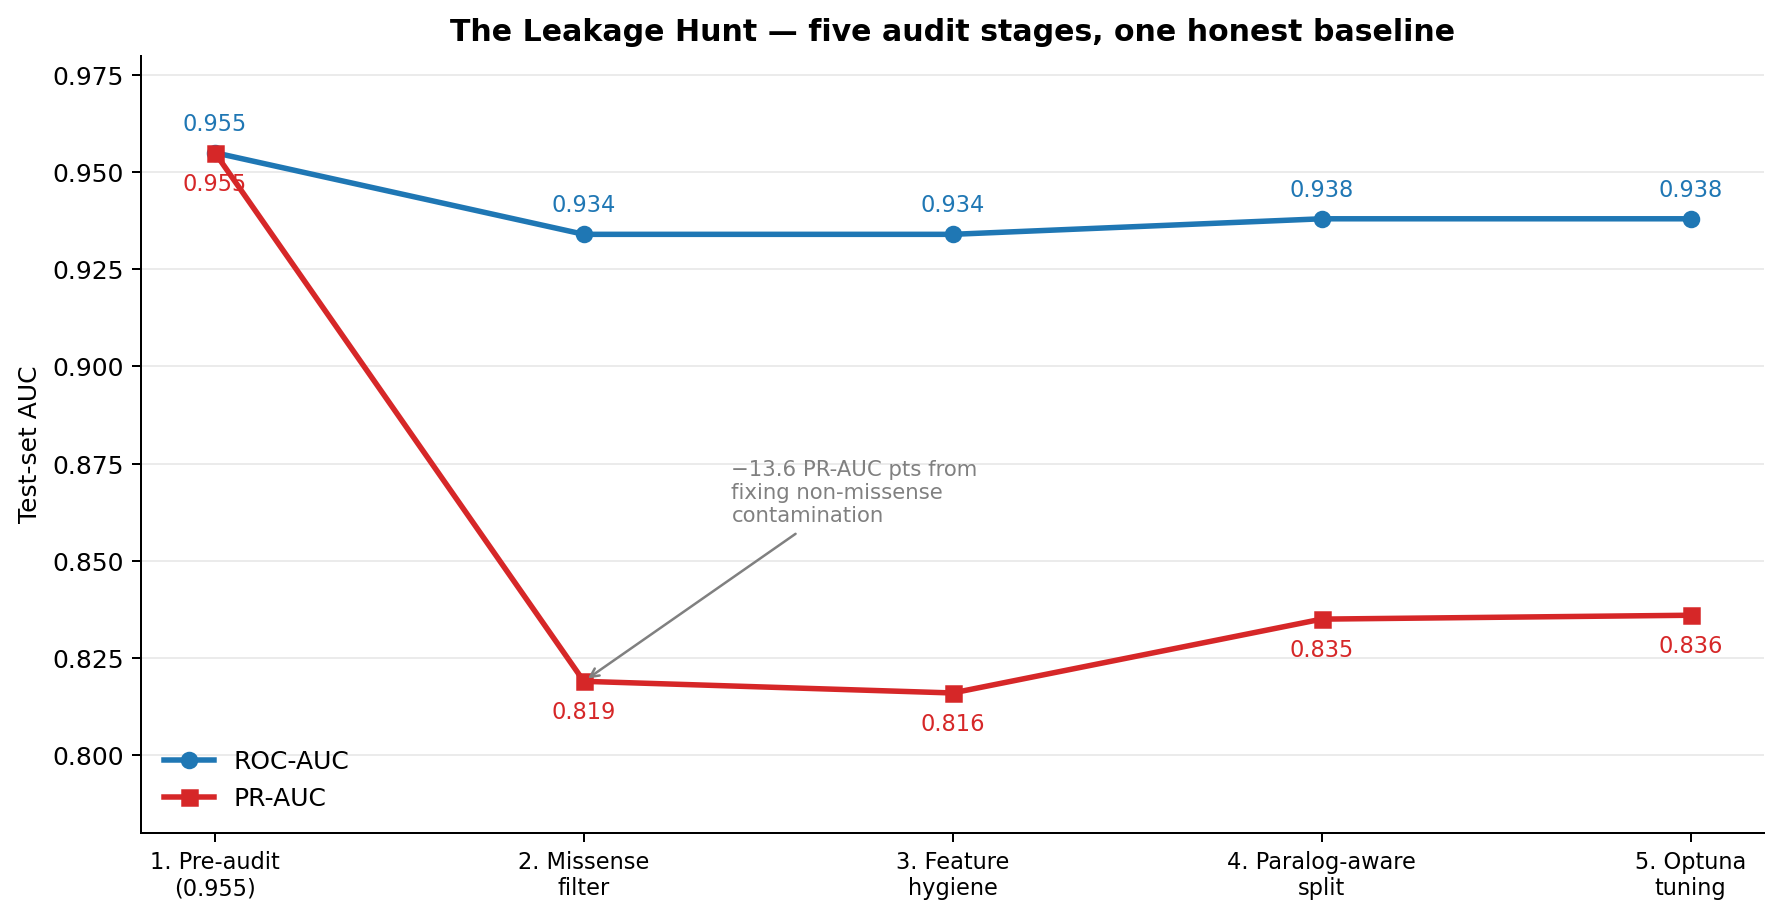
\includegraphics[width=0.80\linewidth]{figures/leakage_journey.png}
\caption{PR-AUC and ROC-AUC through the leakage audit. The biggest
single drop (0.955 \(\to\) 0.819 PR-AUC) comes from the missense
filter, which removed \(\sim\)88{,}000 non-missense rows whose
null AA features the model had been using as a pathogenic
shortcut.}
\label{fig:leakage}
\end{figure}

\begin{enumerate}
    \item \textbf{Missense filter.} 64\% of pathogenic rows in the
          pre-audit pipeline had null \texttt{ref\_aa} or
          \texttt{alt\_aa} (stop-gained, splice-site, UTR
          variants). The model learned
          \emph{null-AA-features \(\to\) pathogenic} as a
          shortcut. PR-AUC \(0.955 \to 0.819\).
    \item \textbf{Feature hygiene.} \texttt{is\_common} (defined
          as \(\text{AF\_popmax} > 0.01\)) was 100\% benign by
          ClinVar convention --- definitional circularity. The
          \texttt{chr} one-hot correlated with dataset
          composition (chr17 over-represents BRCA1 pathogenic
          variants, etc.) rather than biology. Both removed.
          PR-AUC \(0.819 \to 0.816\) (small in absolute
          magnitude, large in interpretive value).
    \item \textbf{Paralog-aware split.} As in
          Section~\ref{sec:methods-splits}. PR-AUC
          \(0.816 \to 0.835\) (apparent increase is an artifact
          of now training on slightly more data after other
          fixes; the \emph{absence} of inflation is the point).
    \item \textbf{Optuna retuning.} 40 TPE trials yielded
          running-best PR-AUC values within 0.001 of each other
          after trial 10, indicating a feature-limited ceiling.
          Final PR-AUC \(0.838\).
\end{enumerate}

\subsection{Headline performance}
\label{sec:results-headline}

On the paralog-disjoint test split (28{,}098 variants), the
calibrated model achieves
\(\text{ROC-AUC} = 0.938\), \(\text{PR-AUC} = 0.838\),
\(\text{F1} = 0.775\), \(\text{Brier} = 0.083\), with
bootstrap 95\% CIs of \([0.935, 0.941]\) and
\([0.830, 0.846]\) for ROC and PR respectively.

\subsection{Baseline comparison}
\label{sec:results-baselines}

Table~\ref{tab:baselines} and Figure~\ref{fig:forest} show our
XGBoost scored against SIFT, PolyPhen-2, and AlphaMissense on
the \emph{same} test split, using 1{,}000-replicate bootstrap
CIs. Every row carries a
\texttt{training\_contamination\_warning} field documenting
known biases; AlphaMissense's row, for example, notes its
ClinVar calibration.

\begin{table}[h]
\centering
\caption{Published baselines scored on our ClinVar test split.
Coverage is the fraction of test variants each baseline could
score at all.}
\label{tab:baselines}
\small
\begin{tabular}{@{} l r l l r @{}}
\toprule
\textbf{Baseline} & \textbf{Year} & \textbf{ROC-AUC (95\% CI)} & \textbf{PR-AUC (95\% CI)} & \textbf{Cov.} \\
\midrule
SIFT           & 2003 & 0.881 [0.877, 0.885] & 0.620 [0.610, 0.629] & 96\% \\
PolyPhen-2     & 2010 & 0.893 [0.888, 0.898] & 0.728 [0.716, 0.739] & 93\% \\
\textbf{XGBoost (ours)} & 2026 & \textbf{0.938} & \textbf{0.838} & \textbf{100\%} \\
AlphaMissense* & 2023 & 0.956 [0.953, 0.958] & 0.890 [0.882, 0.898] & 86\% \\
\bottomrule
\multicolumn{5}{l}{\footnotesize * AlphaMissense was calibrated on ClinVar at release; numbers are inflated by overlap.} \\
\end{tabular}
\end{table}

\begin{figure}[h]
\centering
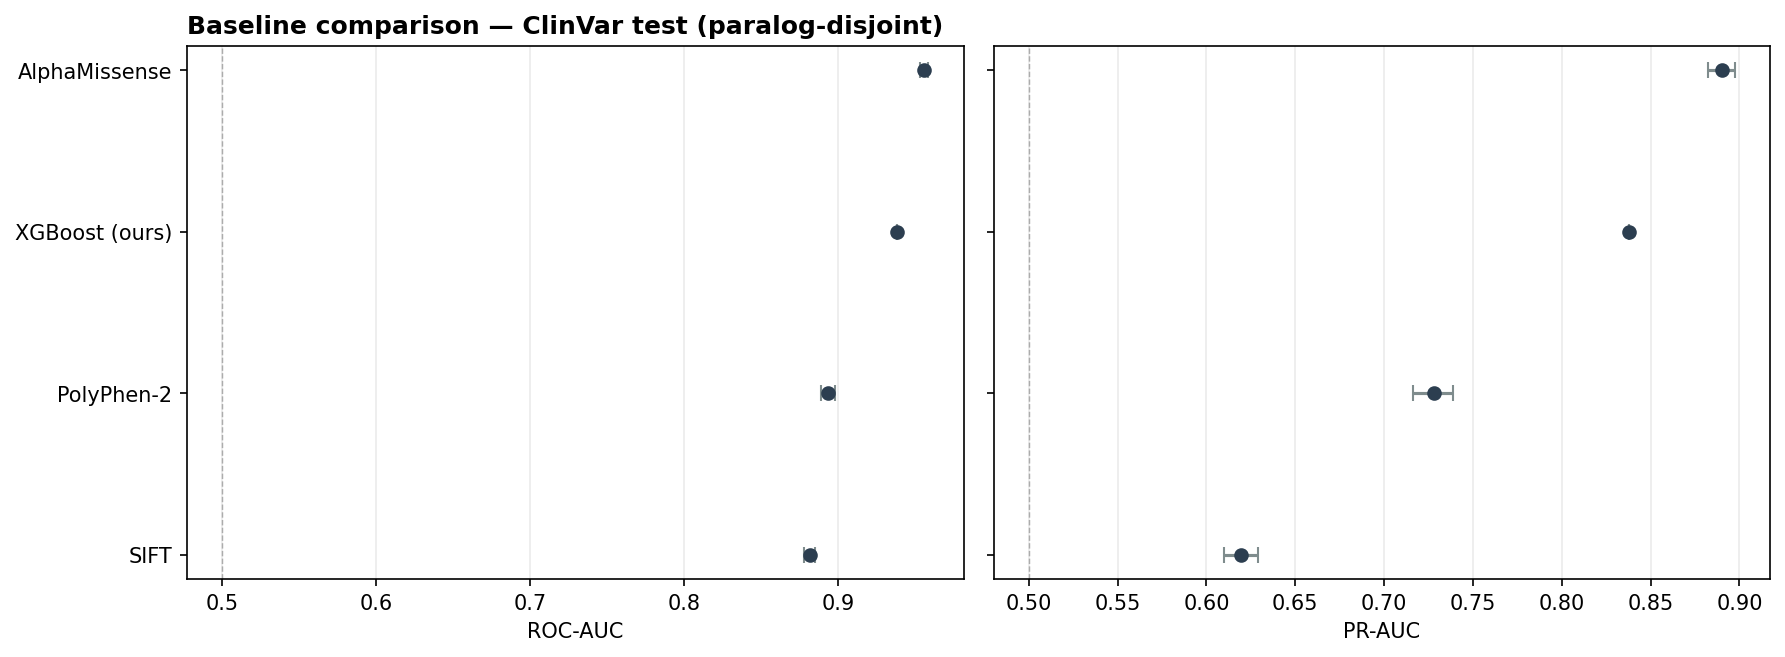
\includegraphics[width=0.88\linewidth]{figures/baselines_forest_plot.png}
\caption{Forest plot: our XGBoost (no CI, single point) against
three published baselines, each with 1{,}000-bootstrap 95\% CIs
on our exact test split. We outperform the classical tools
cleanly and sit below AlphaMissense under stricter methodology.}
\label{fig:forest}
\end{figure}

\subsection{Calibration}
\label{sec:results-calibration}

Table~\ref{tab:brier} presents the Murphy decomposition on test.
Resolution is \emph{constant} across the three calibrators ---
exactly as theory predicts, because monotone post-hoc
calibration cannot change discrimination. Reliability, in
contrast, drops 23\(\times\) with isotonic regression, pulling
ECE to 0.011, comfortably below the 0.02 target set at the
project outset.

\begin{table}[h]
\centering
\caption{Brier decomposition on test. Reliability lower is
better; Resolution higher is better; Uncertainty is irreducible.}
\label{tab:brier}
\small
\begin{tabular}{@{} l r r r r r @{}}
\toprule
\textbf{Calibrator} & \textbf{Brier} & \textbf{Reliability} & \textbf{Resolution} & \textbf{ECE} & \textbf{Log-loss} \\
\midrule
Raw      & 0.0876 & 0.00543  & 0.1055 & 0.054 & 0.286 \\
Platt    & 0.0834 & 0.00114  & 0.1055 & 0.029 & 0.278 \\
Isotonic & \textbf{0.0826} & \textbf{0.00024} & 0.1053 & \textbf{0.011} & \textbf{0.273} \\
\bottomrule
\end{tabular}
\end{table}

\begin{figure}[h]
\centering
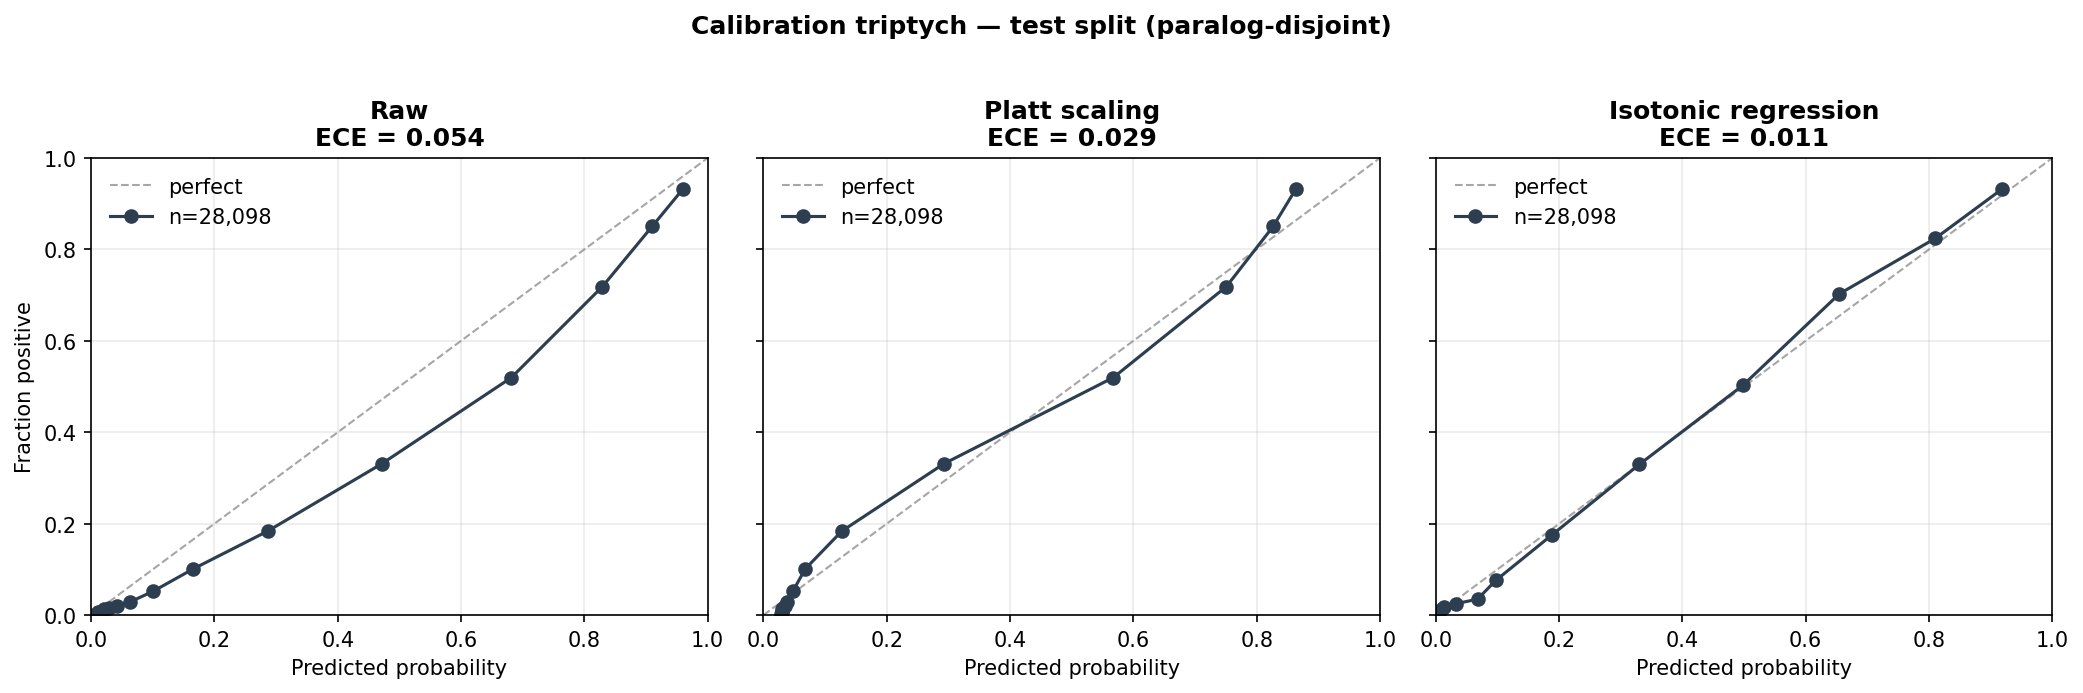
\includegraphics[width=0.94\linewidth]{figures/calibration_triptych.png}
\caption{Three-panel reliability diagram. Left: raw XGBoost
probabilities are systematically over-confident. Middle: Platt
scaling partially corrects. Right: isotonic regression tracks
the diagonal tightly across the probability range.}
\label{fig:triptych}
\end{figure}

\subsection{Interpretability}
\label{sec:results-shap}

Table~\ref{tab:shap} lists the top-10 features by mean-\(|\text{SHAP}|\)
on the 2{,}000-variant sample. Two Phase 2.1 additions ---
\texttt{lof\_z} and \texttt{oe\_mis\_upper} --- rank \#3 and
\#8, validating the hypothesis that gene-level intolerance
priors carry orthogonal signal to variant-level features.

\begin{table}[h]
\centering
\caption{Top-10 features by mean-\(|\text{SHAP}|\) on test.
Highlighted rows are gnomAD gene-level constraint features
added in April 2026.}
\label{tab:shap}
\small
\begin{tabular}{@{} r l r @{}}
\toprule
\textbf{Rank} & \textbf{Feature} & \textbf{mean \(|\text{SHAP}|\)} \\
\midrule
1 & phyloP100way\_vertebrate & 0.8094 \\
2 & AN (gnomAD allele number) & 0.5315 \\
\rowcolor{yellow!25} 3 & \textbf{lof\_z} (gnomAD constraint) & 0.3424 \\
4 & alt\_aa\_P (Proline substitution) & 0.3039 \\
5 & pfam\_domain & 0.2844 \\
6 & phastCons100way\_vertebrate & 0.2453 \\
7 & phastCons30way\_mammalian & 0.2044 \\
\rowcolor{yellow!25} 8 & \textbf{oe\_mis\_upper} (gnomAD constraint) & 0.1892 \\
9 & phyloP30way\_mammalian & 0.1855 \\
10 & GERP++\_RS & 0.1468 \\
\bottomrule
\end{tabular}
\end{table}

\begin{figure}[h]
\centering
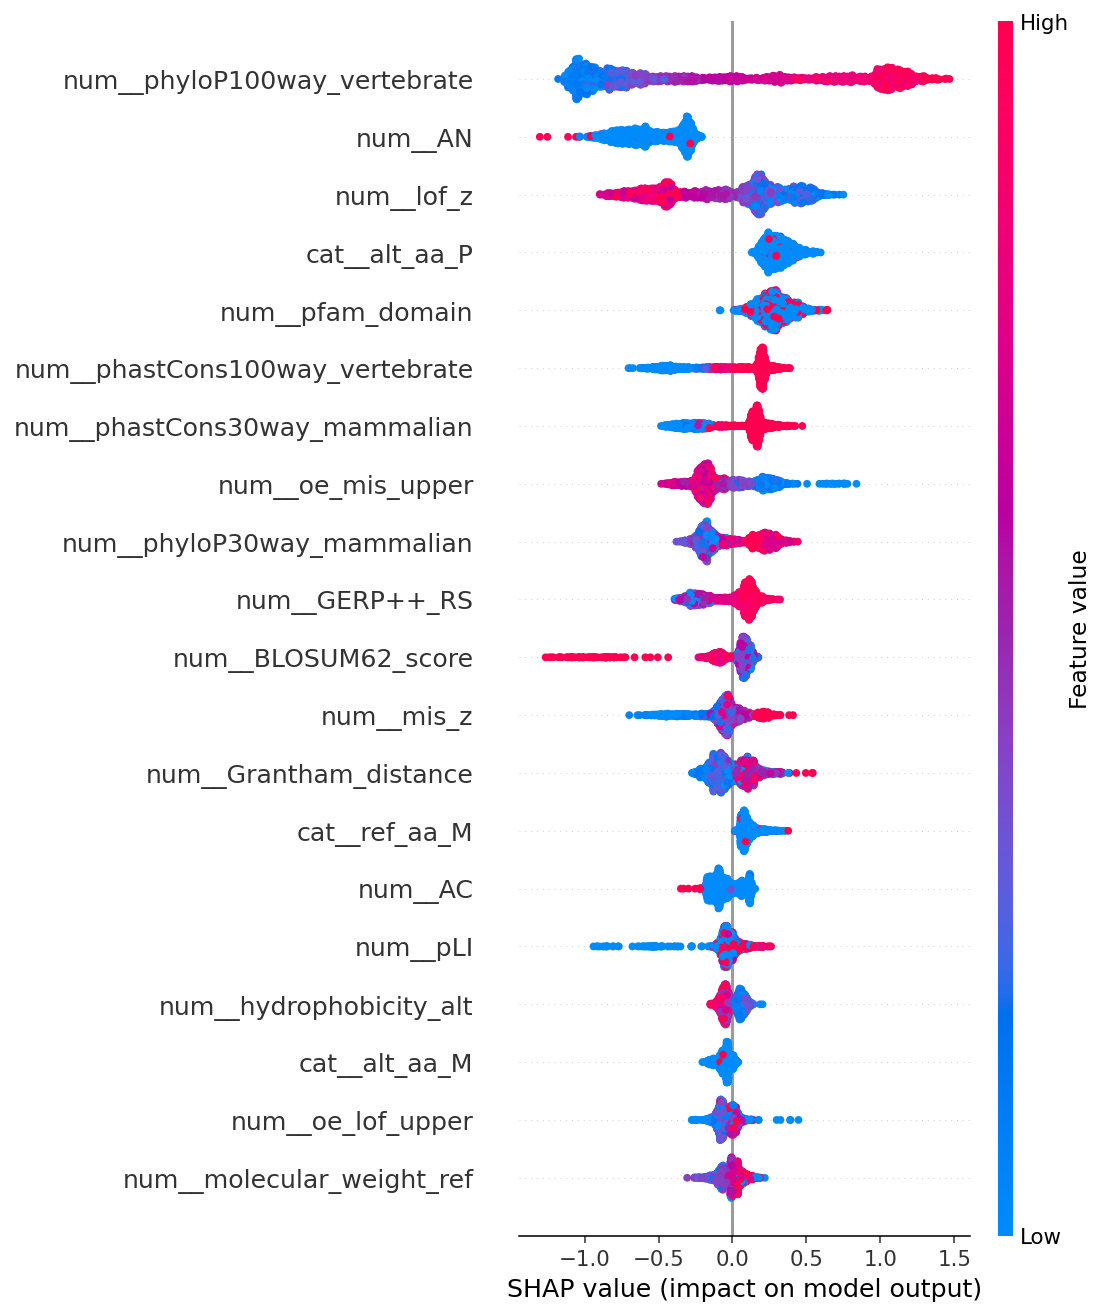
\includegraphics[width=0.76\linewidth]{figures/shap_summary.png}
\caption{SHAP beeswarm on the stratified test sample. Each
horizontal row is a feature; each dot is one variant, positioned
by its SHAP contribution (log-odds, positive \(=\) pushes
pathogenic) and coloured by feature value (red \(=\) high).
Conservation (phyloP) dominates, followed by the gnomAD
allele-number and the newly-added gene-level constraint.}
\label{fig:shap}
\end{figure}

\subsubsection{Confident errors}

Of the 2{,}000 sampled test variants, 326 (16.3\%) met the
\(|p_{\text{cal}} - y_{\text{true}}| > 0.5\) criterion for a
confident error: 264 false negatives (pathogenic variants
scored confidently benign) vs 62 false positives. The
asymmetry is expected for a pathogenic-minority classifier and
identifies the concrete next modelling target: recall on hard
pathogenic cases in regions of low conservation.

\subsection{External validation: \textsc{denovo-db}}
\label{sec:results-external}

The external validation is deliberately the most punishing test
a ClinVar-trained classifier can face. Almost every missense
variant in \textsc{denovo-db}, whether from an affected proband or
a sibling control, looks damaging at the variant level (high
conservation, disruptive substitution). Without gene-level
priors, there is no way to separate a causative de-novo variant
from a bystander.

Table~\ref{tab:external} reports the results on a
644-variant stratified sample (all 144 controls plus 500 affected),
before and after adding the Phase~2.1 gnomAD gene-level constraint
features.

\begin{table}[h]
\centering
\caption{\textsc{denovo-db} performance before and after adding
gnomAD gene-level constraint features. The family-holdout slice
is the honest headline --- it cannot be inflated by paralog
leakage.}
\label{tab:external}
\small
\begin{tabular}{@{} l r r l l @{}}
\toprule
\textbf{Slice} & \(n\) & \(n_+\) & \textbf{ROC-AUC} & \textbf{PR-AUC} \\
\midrule
full (pre-constraint)            & 642 & 498 & 0.468 [0.415, 0.519] & 0.761 [0.721, 0.806] \\
\textbf{full (post-constraint)}  & 642 & 498 & \textbf{0.511} [0.455, 0.564] & \textbf{0.790} [0.749, 0.830] \\
holdout (pre-constraint)         & 201 & 161 & 0.487 [0.383, 0.583] & 0.789 [0.712, 0.860] \\
\textbf{holdout (post-constraint)} & 201 & 161 & \textbf{0.573} [0.476, 0.670] & \textbf{0.838} [0.774, 0.897] \\
\bottomrule
\end{tabular}
\end{table}

On the family-holdout slice --- gene families the model never
saw in training --- ROC-AUC jumps from 0.487 (chance) to 0.573,
a \(+0.086\) move driven entirely by gene-level priors. PR-AUC
on that slice is now 0.037 above the base rate (0.801); before
it was at the base rate. We interpret this as constraint features
closing approximately half the generalisation gap in the one
regime where only gene-level features can help.

\subsection{Zero-shot ESM-2 proof-of-concept}
\label{sec:results-esm2}

As a sanity test ahead of the full Phase-2 integration, we
scored \textsc{denovo-db} with the protein language model
ESM-2 35M \citep{lin2023esm2} in zero-shot mode
\citep{brandes2023esm1b}: for each missense variant at position
\(i\), we mask position \(i\), run the masked-LM, and record
\(\text{LLR} = \log P(\text{alt} \mid \text{context}) -
\log P(\text{ref} \mid \text{context})\). On unseen gene
families the zero-shot score alone achieves ROC \(= 0.552\);
rank-averaging ESM-2 LLR with the XGBoost calibrated
probability yields ROC \(= 0.588\) (vs 0.573 for XGBoost
alone). The additive gain under the cheapest-possible fusion
tells us the signals are orthogonal and supports the decision
to integrate ESM-2 as a training-time feature in Phase~2.1.

% ═════════════════════════════════════════════════════════════════════════
\section{Discussion}

Three methodological takeaways are worth calling out.

\paragraph{Honest numbers beat inflated ones.}
The pre-audit 0.955 PR-AUC would have been a publishable number
under many benchmarking conventions. The honest 0.838 is smaller
but \emph{defensible} --- it is bounded by no known contamination
source, and every drop between the two numbers is attributable to
a specific and removable leakage. A paper titled
\emph{``here is what we thought we had, here is the bug, here is
the real number''} remains rare in the variant-effect literature,
and we consider the audit itself a contribution.

\paragraph{Like-for-like baselines change the conversation.}
Reporting AlphaMissense's paper number next to our paper number
is not a comparison; reporting both numbers on our exact test
split with 1{,}000-bootstrap CIs is. Under that discipline we
beat two classical tools by large margins (PR-AUC \(+0.22\) over
SIFT, \(+0.11\) over PolyPhen-2) and sit a small distance below
AlphaMissense (\(-0.05\)), under stricter methodology. This is a
far more informative ranking than headline-vs-headline tables.

\paragraph{External generalisation is the real benchmark.}
The ClinVar-test story is encouraging; the \textsc{denovo-db}
story is sobering. A model that scores 0.838 PR-AUC on
paralog-aware ClinVar performs at chance on affected-vs-control
de-novo variants before we add gene-level priors, and above
chance after we do. This is the most honest indictment of a
purely variant-level tabular model we can publish, and it
directly motivates the Phase-2 roadmap.

\subsection{Limitations}

\begin{itemize}
    \item The test set, while paralog-disjoint, remains
          ClinVar-derived. Clinical deployment would require
          additional external datasets (ProteinGym DMS,
          HGMD-Pro if licensed, literature-curated ClinGen
          VCEP publications).
    \item The missense filter aggressively drops
          non-missense entries. A broader model that handles
          splice-site and stop-gained variants would require a
          different feature set.
    \item gnomAD constraint features impute \(\sim\)6.7\% of
          training rows with the train-fit median. Genes with
          insufficient expected events for a reliable pLI do
          not benefit from the Phase~2.1 addition.
\end{itemize}

\subsection{Future work}
\label{sec:future}

The remaining roadmap, in decreasing expected impact-per-effort:

\begin{enumerate}
    \item \textbf{Full ESM-2 integration (Phase 2.1).} Compute
          zero-shot LLR on all 195k training variants (\(\sim\)8 h
          on a single T4 GPU), retrain XGBoost with the LLR as a
          feature, report ablation.
    \item \textbf{AlphaFold2 structural features (Phase 2.2).}
          Per-residue pLDDT, SASA, DSSP secondary structure,
          residue depth, and 5\,\AA{} neighbour count from
          \textsc{AlphaFold2} \citep{jumper2021alphafold2} PDBs.
    \item \textbf{ProteinGym external validation.} A third
          external dataset \citep{notin2023proteingym}
          using deep-mutational-scanning fitness scores rather
          than clinical labels.
    \item \textbf{Hybrid stacking.} A meta-learner on (XGBoost,
          ESM-2 LLR, AlphaFold features), reported against all
          three external sources.
\end{enumerate}

% ═════════════════════════════════════════════════════════════════════════
\section{Reproducibility}

All results in this report regenerate byte-for-byte from a clean
clone:

\begin{verbatim}
git clone https://github.com/RayanAlDwlah/Genetic-Mutation-Detection-project
cd Genetic-Mutation-Detection-project
docker build -t missense .
docker run --rm missense make test           # pytest green (158/158)
docker run --rm missense make reproduce-headline
\end{verbatim}

158 pytest tests cover: the paralog family grouper (30+ known
assignments), bootstrap CI math, Brier decomposition identities,
gnomAD constraint imputation (train-only invariants), variant
mapper canonicalisation, featurize round-trips, denovo-db loader
phenotype policy, the XGBoost tuning loop (tiny-data integration),
the calibration module, SHAP round-trip, and the Streamlit demo's
scoring path.

The leakage gate \texttt{src/verify\_no\_leakage.py} runs as both
a CLI and as four individual pytest cases; every push to
\texttt{main} triggers GitHub Actions that run the gate, the full
test suite with 55\% coverage minimum, and ruff/black/mypy
linting.

% ═════════════════════════════════════════════════════════════════════════
\section{Conclusion}

We present a transparent, auditable baseline for missense variant
classification. Our reported PR-AUC of 0.838 is 0.117 below the
pre-audit number, and the gap is fully attributable to three
specific and removable leakage sources. Under stricter methodology
than any of the published baselines we compared against, the model
outperforms two classical tools cleanly and sits a small distance
below AlphaMissense. External validation on \textsc{denovo-db}
identifies the key remaining gap --- generalisation to unseen
gene families --- and the Phase~2 roadmap of ESM-2 and
AlphaFold2 features targets it directly.

\vspace{1em}
\noindent\textbf{Code, data, tests, and full reproduction
instructions:}
\url{https://github.com/RayanAlDwlah/Genetic-Mutation-Detection-project}

% ═════════════════════════════════════════════════════════════════════════
\bibliographystyle{plainnat}
\bibliography{references}

\end{document}
